\documentclass[pdftex,12pt,a4paper]{article}
\usepackage[pdftex]{graphicx}
\usepackage{xcolor}
\usepackage{marginnote}
\usepackage{enumitem}
\usepackage[bottom=1.5cm, outer=5cm, inner=2cm, heightrounded,
marginparwidth=4cm, marginparsep=0.5cm]{geometry}

\begin{document}
    % Custom title page
    \begin{titlepage}
        \begin{center}
            
\includegraphics[width=5cm]{figures/kulogo}\\[1cm]
            {\Large \bfseries
                Spring 2014\\
                Computer Networks\\
                CMPE323\\[1cm]
            }
            {\large \bfseries
                \noindent Laboratory Experiment No. 3: Introduction to VLANs\\[1cm]
            }
        \end{center}

        \noindent \textbf{Aims and Objectives:}
            \begin{itemize}[leftmargin=4cm]
                \item Introduce students to Virtual Local Area Networks (VLANs),
                \item the general semantics of VLANs within a switch,
                \item the general semantics of VLANs between switches,
                \item and the structure of IEEE 802.1Q tags which allows for
                    maintaining inter-switch VLAN separation.
            \end{itemize}
            \vspace{0.5cm}

        \noindent \textbf{Materials Required:}
            \begin{itemize}[leftmargin=4cm]
                \item Ethernet switches,
                \item PCs with Ethernet adapters,
                \item and Straight-through/crossover/rollover cables.
            \end{itemize}
            \vspace{0.5cm}

        \noindent \textbf{Change Log:}
            \begin{itemize}[leftmargin=4cm]
                \item 3-3-2014: original document -- mkhonji.
            \end{itemize}
    \end{titlepage}
    \newpage

    % Lab script content
    \section{Introduction}
        \subsection{Limitations in the previous lab}
            The following limitations existed in the previous lab\footnote{Lab 2:
            Introduction to Ethernet Networks}:
            \begin{itemize}
                \item Broadcast domain limitations --- each switch formed a single
                    broadcast domain where \emph{unknown unicast}\footnote{MAC
                    packets with destination MAC addresses that do not exist in the
                    MAC address table of the forwarding switch} and
                    \emph{broadcast}\footnote{MAC packets with destination MAC
                    addresses of \texttt{FF:FF:FF:FF:FF:FF}.} messages were forwarded to
                    all connected ports on the same Ethernet switch.  This can cause
                    efficiency\footnote{Efficiency problems as excessive messages can
                    consume the link bandwidth, specially when the broadcast domain
                    is large.} and security\footnote{Some attacks can be performed only
                    when the attacker resides in the same broadcast domain as the
                    victim; e.g. MAC address table spoofing, and ARP spoofing.}
                    issues.
                \item Management limitations --- in order to have separate
                    broadcast domains, separate physical switches were used, and in
                    order to relocate a PC from one broadcast domain into another,
                    we had to physically disconnect it from one switch and
                    physically connect it to another switch.
            \end{itemize}

        \subsection{A solution to the limitations}
            In this lab, by using Virtual LANs (VLANs), you will learn how to
            address the two limitations that existed in the previous lab as
            follows:
            \begin{itemize}
                \item Fine-grained broadcast domains --- by assigning groups of
                    switch ports to different VLANs, you essentially create
                    different broadcast domains within a single switch. Although
                    this is virtual (by software configuration), it is practically
                    the same as using separate physical switches from the
                    perspective of the connected nodes (or PCs).
                \item Easier management --- when a network administrator wishes to
                    relocate one PC from a broadcast domain into another, all what
                    is needed is changing the software configuration of the switch
                    port such that its VLAN membership is updated to the desired
                    one. In other words, we no longer need to physical
                    disconnect/connect cables in order to relocate nodes (or PCs)
                    from one broadcast domain into another.

                    Additionally, it is possible to maintain the semantics of such
                    virtual broadcast domains across multiple Ethernet switches.
                    Since broadcast domains have identifiers (i.e. VLAN ID), a
                    special connection\footnote{A connection between two switches
                    that accepts tagged MAC frames by IEEE 802.1Q tags.} between
                    two switches allows MAC frames of different VLANs to be tagged
                    accordingly when being transmitted to other switches, so that
                    the switches can maintain broadcast domain isolation based on
                    such VLAN IDs (as the IDs are communicated by the MAC frame
                    IEEE 802.1Q tags).
            \end{itemize}

        \subsection{Specifications of the IEEE 802.1Q tag}
            The standard IEEE 802.1Q defines an Ethernet tag that facilitates the
            following:
            \begin{itemize}
                \item A new \texttt{Type} field is added. It must have the value of
                    \texttt{0x8100} in order to indicate that there are 2
                    proceeding octets describe Tag Control Information as
                    depicted in Figure \ref{fig:macpacket} --- under the scope
                    of this lab.
                \item A set of bits to convey the VLAN ID. As depicted in Figure
                    \ref{fig:dot1q}, there are 12 bits that are assigned to
                    specify the VLAN ID.  --- under the scope of this lab.
                \item A set of bits to describe the priority of the MAC frame
                    which helps later in Quality of Service (QoS) tasks ---
                    Priority Code Point (PCP) and Discard Eligibility (DE) are
                    beyond the scope of this lab.
            \end{itemize}
            
            \begin{figure}[tbh]
                \centering
                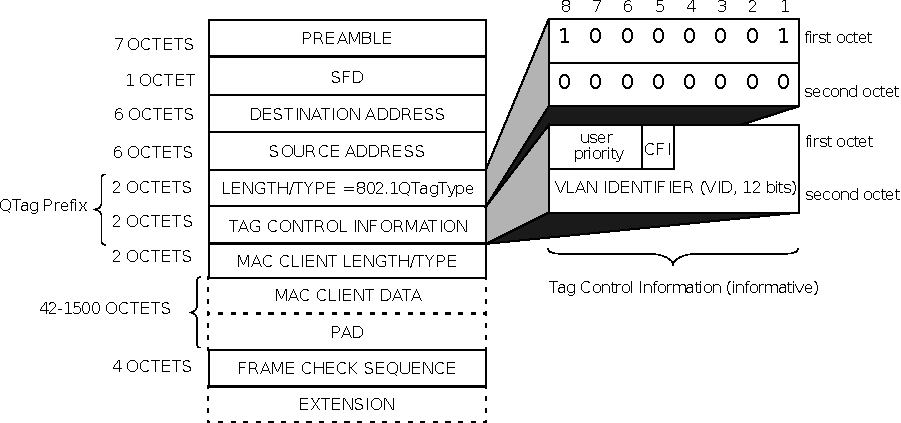
\includegraphics[width=0.9\textwidth]{figures/macpacket}
                \caption{MAC packet example with a IEEE 802.1Q tag --- Source: IEEE Std.
                802.1Q-2011, Annex G.1.}
                \label{fig:macpacket}
            \end{figure}

            \begin{figure}[tbh]
                \centering
                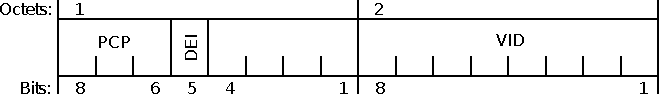
\includegraphics[width=0.7\textwidth]{figures/dot1q}
                \caption{VLAN Tag Control Information (TCI) --- Source: IEEE Std.
                802.1Q-2011, Section 9.6.}
                \label{fig:dot1q}
            \end{figure}

    \section{Lab Preparation}
        \begin{itemize}
            \item Setup the lab topology as depicted in Figure
                \ref{fig:netdiag}.
            \item Reboot all the lab PCs\footnote{Use the \texttt{reboot}
                command in case you are using Linux PCs.}.
            \item Erase\footnote{Using the command \texttt{erase
                startup-config}.} the configuration of the switches, and then
                reboot\footnote{Using the command \texttt{reload}.} them.
            \item Run WireShark on all the involved PCs.
        \end{itemize}

        \begin{figure}[tbh]
            \centering
            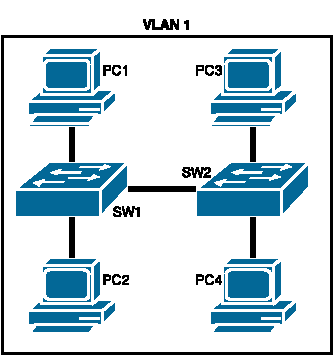
\includegraphics[width=0.45\textwidth]{figures/netdiag}
            \caption{Initial lab network diagram.}
            \label{fig:netdiag}
        \end{figure}

    \section{Lab experiments}
        \subsection{A single broadcast domain}
            \begin{flushright}
                \textbf{[20 points]}\marginnote{\small \textbf{Note:} When done, show your
                work to the lab engineer for grading purposes.}
            \end{flushright}

            Using \texttt{scapy} or the provided C code, broadcast the
            following MAC packet:
            \begin{itemize}
                \item Source MAC address:
                    \texttt{00:00:00:00:00:0X}\footnote{\texttt{X} is your PC
                    ID (e.g. PC1 will have the MAC address
                    \texttt{00:00:00:00:00:01}).}.
                \item Destination MAC address (broadcast): \texttt{FF:FF:FF:FF:FF:FF}.
                \item Data type: \texttt{0x05FF}\footnote{You are free to choose any
                    other valid value for the \texttt{Type} field.}.
                \item Payload data: \texttt{TeamY}\footnote{Y is your team ID. For
                    example, for team 1 you would send octets \texttt{0x54,
                    0x65, 0x61, 0x6D, 0x31}.}.
            \end{itemize}

            Then answer the following questions:
            \begin{enumerate}
                \item List the PC IDs that received the MAC packet that you
                    have sent earlier.
                \item Logically thinking, list problems that can arise if many
                    more Ethernet switches are interconnected to form a large
                    broadcast domain.
            \end{enumerate}


        \subsection{Virtually separated broadcast domains}
            \begin{flushright}
                \textbf{[40 points]}\marginnote{\small \textbf{Note:} When done, show your
                work to the lab engineer for grading purposes.}
            \end{flushright}

            As depicted in Figure \ref{fig:netdiag2}, re-configure the network
            as follows:
            \begin{enumerate}
                \item In switches \texttt{SW1} and \texttt{SW2},
                    create\footnote{Using the commands \texttt{enable},
                    \texttt{configure terminal}, \texttt{vlan 100}, and
                    \texttt{vlan 200}} VLANs 100 and 200.
                    \texttt{SW2}.
                \item In switches \texttt{SW1} and \texttt{SW2},
                    assign\footnote{Using the commands \texttt{enable},
                    \texttt{configure terminal}, \texttt{interface FastEthernet 0/A}, and
                    \texttt{switchport access vlan B}, where \texttt{A} is the
                    interface that ID, and \texttt{B} is the VLAN ID.} PC1 \& PC3 to
                    VLAN 100, and PC2 \& PC4 to VLAN 200.
            \end{enumerate}

            \begin{figure}[tbh]
                \centering
                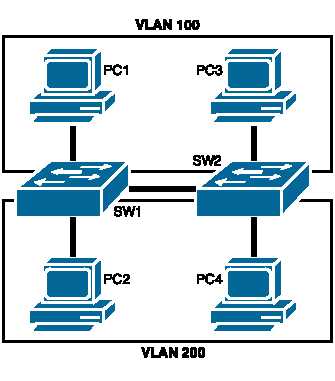
\includegraphics[width=0.45\textwidth]{figures/netdiag2}
                \caption{Lab network diagram with VLANs.}
                \label{fig:netdiag2}
            \end{figure}

            Then answer the following questions:
            \begin{enumerate}
                \item Send a broadcast MAC packet from PC1, then list the PCs
                    that received the MAC packet.
                \item Send a broadcast MAC packet from PC2, then list the PCs
                    that received the MAC packet.
                \item Send a broadcast MAC packet from PC3, then list the PCs
                    that received the MAC packet.
                \item Send a broadcast MAC packet from PC4, then list the PCs
                    that received the MAC packet.
                \item Based on the tests above, what do you conclude with
                    regards to the scope of the broadcast domain?
            \end{enumerate}

        \subsection{Analyze IEEE 802.1Q tags}\label{sec:analyze}
            \begin{flushright}
                \textbf{[40 points]}\marginnote{\small \textbf{Note:} When
                done, show your work to the lab engineer for grading purposes.}
            \end{flushright}

            Connect your laptop\footnote{You may use a desktop PC if
            available.} to your team's switch as depicted in Figure
            \ref{fig:netdiag3}, run WireShark on your laptop, then configure a
            monitoring session in your team's switch as follows:
            \begin{itemize}
                \item Configure the trunk port of your team's switch as a
                    monitoring source\footnote{Using the commands
                    \texttt{enable}, \texttt{configure terminal},
                    \texttt{monitor session 1 source interface FastEthernet 0/T},
                    where \texttt{T} is the trunk port ID.}.
                \item Configure the laptop's port as a monitoring
                    destination\footnote{Using the commands \texttt{enable},
                    \texttt{configure terminal}, \texttt{monitor session 1
                    destination interface FastEthernet 0/L}, where \texttt{L} is the
                    port that connects to the monitoring laptop.}.
            \end{itemize}

            \begin{figure}[tbh]
                \centering
                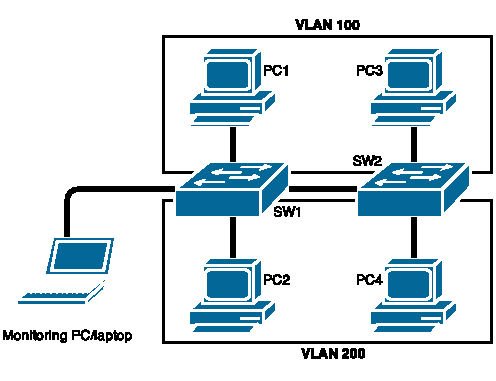
\includegraphics[width=0.7\textwidth]{figures/netdiag3}
                \caption{Lab network diagram with VLANs after connecting the
                monitoring PC/laptop.}
                \label{fig:netdiag3}
            \end{figure}

            Then answer the following questions:
            \begin{enumerate}
                \item Send a broadcast MAC packet from PC1, then view the
                    WireShark instance on the monitoring laptop to analyze the
                    IEEE 802.1Q tag. What is the content of the tag?.
                \item Send a broadcast MAC packet from PC2, then view the
                    WireShark instance on the monitoring laptop to analyze the
                    IEEE 802.1Q tag. What is the content of the tag?.
                \item Send a broadcast MAC packet from PC3, then view the
                    WireShark instance on the monitoring laptop to analyze the
                    IEEE 802.1Q tag. What is the content of the tag?.
                \item Send a broadcast MAC packet from PC4, then view the
                    WireShark instance on the monitoring laptop to analyze the
                    IEEE 802.1Q tag. What is the content of the tag?.
                \item Based on the observations earlier, how can
                    inter-connected Ethernet switches maintain VLAN separation
                    of frames?
            \end{enumerate}

        \subsection{Extra questions (not graded)}\marginnote{\small
            \textbf{Note:} when done, show your answers to the lab engineer for
            feedback. If the lab time is not enough, take your time and submit it
            in a later time. Although not graded, it can strengthen your
            understanding of the subject.}

            In this section, you will be able to use your laptop to inject MAC
            packets into various VLANs.

            \begin{enumerate}
                \item Remove the monitoring session that you have configured
                    earlier in Section \ref{sec:analyze}, and instead,
                    configure the port \texttt{FastEthernet 0/L} as a trunking
                    port.

                \item Then, using your understanding of the format of IEEE
                    802.1Q tags, craft a message from the laptop such that you
                    are able to send a message to targeted VLAN.

                    For example, send a message from your laptop (which is connected to
                    the trunk port) to VLAN 100 and test if PCs in VLAN 100 receive the
                    message. Then, repeat it with VLAN 200 and test if PCs in VLAN 200
                    can receive the message.
            \end{enumerate}

            \subsubsection{Discussion}
                In this task, you were able to gain access to all VLANs after
                configuring the switchport that faces your laptop as a trunking
                port. Which is not necessarily a security threat as the trunking port
                configuration was manual after having physical access to the
                switch, which is usually only available to authorized personnel.

                However, since Cisco switches run an insecure setup of VLAN
                Trunking Protocol (VTP)\footnote{A protocol that allows
                switches to negotiate in order to automatically create
                trunking interfaces.} by default, it is possible to enable such
                trunking ports automatically from your PC/laptop.

                This is why it is recommended to disable VTP on ports that face end
                users PCs (access ports), and secure VTP negotiations with
                passwords when facing other switches.

                \textbf{Note:} VTP is a Cisco-specific protocol and other vendors
                may not have similar protocols. In this lab, we did not have to
                explicitly configure trunking ports because VTP allowed the
                automatic creation of such trunking ports. However, if VTP was
                disabled, then the trunking ports will have to be configured
                manually.
\end{document}
